% Documentclass options:
%    10pt, 11pt, 12pt  -- set type size
%    draft             -- single space, mark overfull hboxes on paper
%    final             -- double space, don't mark overfull hboxes on paper
%    oneside           -- format for one-sided printing
%    twoside           -- format for two-sided printing
% Defaults are 11pt,final,oneside.  Keep these, please.
\documentclass[11pt]{ucscthesisbs}
\bibliographystyle{apalike2}
\usepackage{natbib}
\usepackage{graphicx,epsf}% Include figure files
\usepackage{pgfplots} %for doing graphics within latex!

% The following declaration is for citations and bibliographies consistent with
% Astrophysical Journal specifications.  It may be left out or replaced with
% another bibliography/citation style.  See also the "\bibliographystyle"
% command later in this file.
%\usepackage{apj}

\usepackage{xcolor}
\usepackage{pagecolor}
\usepackage{lipsum}  

\pagecolor{darkgray}
% \pagecolor{black}
\color{white}

\begin{document}

% Declarations for Front Matter

\title{formation of water condensation zones in the atmosphere of uranus and their impact on its thermal evolution}
\author{Robert Schroder}
\degreeyear{2020}
\degreemonth{27 November}
\degree{BACHELOR OF SCIENCE}
\field{ASTROPHYSICS}%
% Declare up to five committee members.  The text will be reproduced directly
% on the signature page.  Though the chair is a committee member, leave
% him/her out of the \committeemember declarations.  Make sure \numberofmembers
% agrees with the number of committee members declared INCLUDING the chair.
% If it is wrong, you will get extra or missing lines on the signature page.
%
\chair{Professor Michael Dine}
\technicaladvisor{Christopher Mankovich}


\campus{Santa Cruz}

\maketitle
\copyrightpage

\begin{frontmatter}

\begin{abstract}
The abstract is a brief but {\it quantitative} summary of all your main results.  It is not an introduction, and it is not a part of your thesis text.  You should assume that someone reading the abstract learns the essentials of what they would learn from reading your whole thesis; and you should assume that someone reading the thesis has not looked at the abstract.  The abstract should be written last, so that it is an accurate summary of what you have written.
\end{abstract}

\tableofcontents
%
% The most recent (10/95) guidelines make absolutely no mention of the list
% of figures and list of tables.  Are they necessary?  If not, comment the
% next two lines out.
%
\listoffigures
\listoftables

\begin{dedication}
\null\vfil
{\large
\begin{center}
To my parents,\\\vspace{12pt}
V. Boson and T. Lepton
\end{center}}
\vfil\null
\end{dedication}

\begin{acknowledgements}
I would like to thank my thesis advisor, maybe my 182 instructor too, or, if I'm not feeling it, my family and friends, or even no one at all (this section is optional).  The dedication is optional too (you can just comment out or delete either of these environments).  However, if your work has been supported by your advisor's research grant, it is customary to acknowledge the financial support here.
\end{acknowledgements}


\end{frontmatter}

%\part{First Part}

\chapter{Introduction}

This is mostly a demonstration of all the mechanics (references, sections, figures, tables, etc.) of a physics senior thesis, but it also includes an incomplete sampling of advice, because we have to say something.  Your notes from Physics 182 are of course a better and more complete discussion of what is required of the thesis.

The first part of the introduction should always quickly state what problem you are planning to solve (or question you are trying to answer) and (if you are doing original research) what methods you are going to use.  For a literature review, the method is obvious -- reading stuff -- but you should still have a central question you want to be gathering evidence to answer.  Once you have done this, your readers will know {\it why} they are going to read the rest of the introductory material.


\section{This demonstrates a section and includes a figure}

It's best to break your chapters up into sections, and, when the topic of a section is long and complicated, even subsections.  Once a section or subsection has gone on for more than about 4 paragraphs, consider whether it might be clearer to break it up (not that this will always be the case).

\begin{figure}[t!]
 \centerline{
  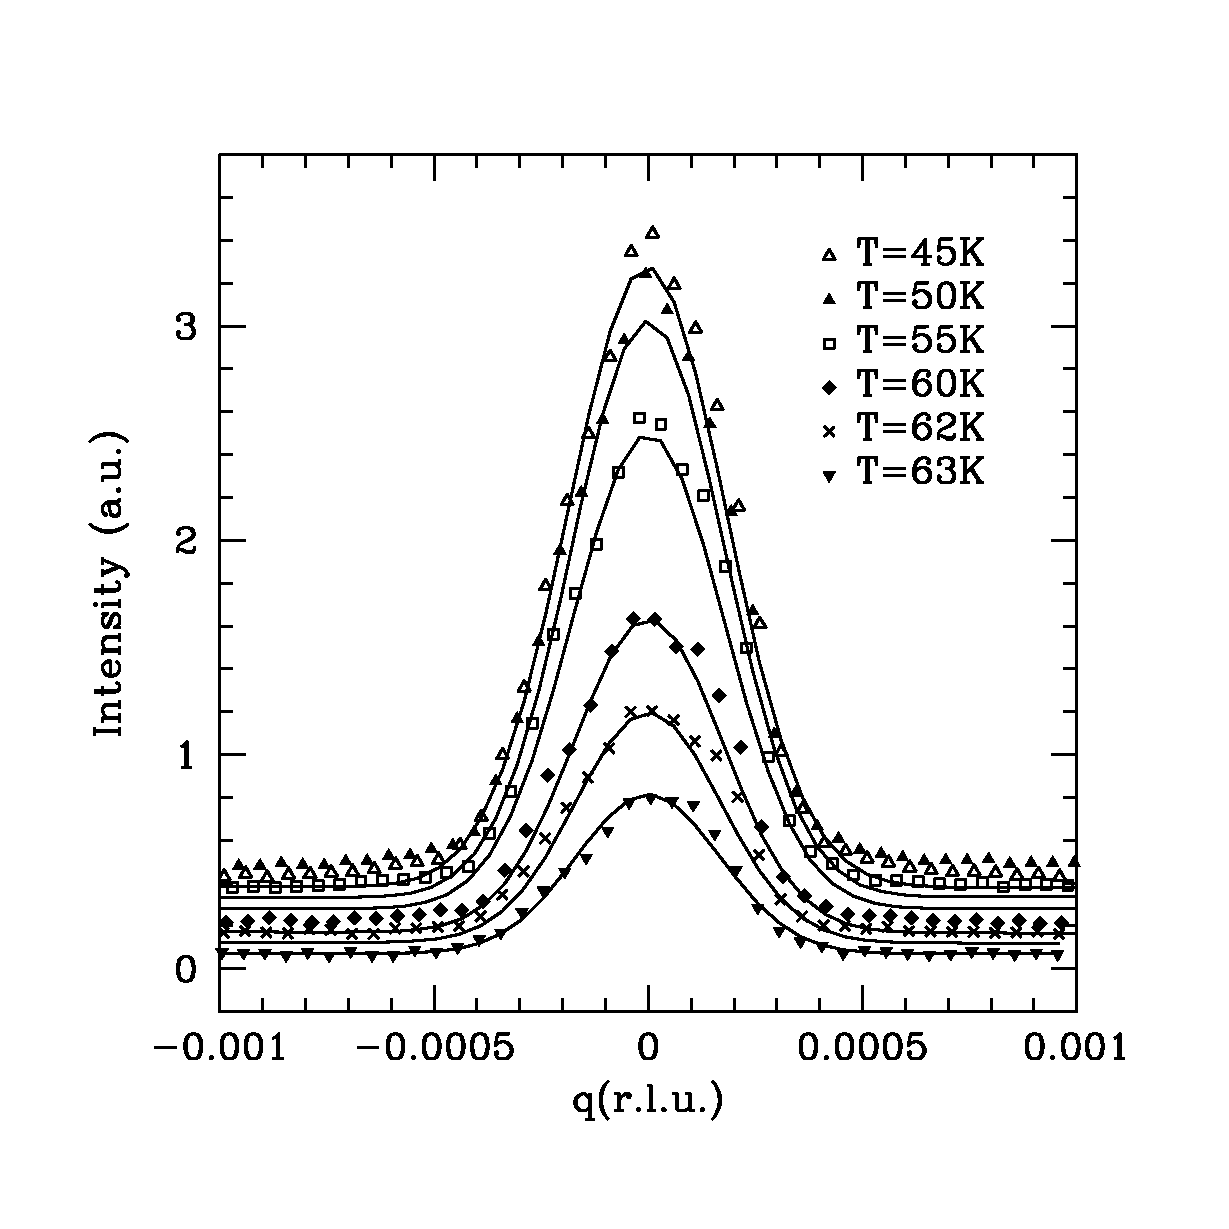
\includegraphics[width=4.0in]{comparezfc_bw.eps}
 }
\caption[Transverse Scans at difference Temperatures at $H=11$~T]
{Representative transverse scans for the different temperatures
below $T_{\rm c}(H) = 63.7$~K taken with
$H=11$~T after cooling in $H=0$. Each scan is displaced vertically by 0.1 units
from the scan below it for clarity.  The solid curves
are results of least-squares fits to
a Gaussian line shapes with a half-width-at-half-maximum
equal to $2.1\times10^{-4}$ r.l.u.  
}
\label{fig:discretescan}
\end{figure}

This section contains a figure that is an encapsulated postscript file, and I reference it by referring to it by its label (like this: see Figure~\ref{fig:discretescan}).  Note that the "label" command in the figure environment has to come after the caption but before the close of the figure environment.  The opposite is true for sections and subsections, where the label appears just after the section/subsection begins (like this: see section~\ref{subsection_example}).  Note that you must reference every figure you include somewhere in text.  And never say "above", "below", etc. for the placement of the figure; instead cite it by its label as demonstrated at the start of this paragraph.  Note that the position of the figure in the processed document doesn't exactly match its position here in the raw text!

\subsection{A subsection, with a discussion of references}\label{subsection_example}

When you cite a reference as the source for a piece of information,
you generally place it just after you give the information, using the "citep"
command \citep{awwzml06}.  However, sometimes you want to refer directly to 
the authors, as \citet{agcs89} did several times, in which case you use "citet".
We are using the American Psychological Association conventions for citations
(what appears in the text) and references (what appears in the bibiography in
the end).  Of course every citation must correspond to a reference and vice versa.

\subsection{Another subsection, with a discussion of equations}\label{subsection_equations}

We can do equations like this first famous attempt
at special relativity $E=ma^2$.  A second attempt
was $E=mb^2$.  Finally, the correct answer was found
to be
However, a pathetic attempt was made to push
for
\begin{equation}
E=mc^{2}
\end{equation}
\noindent but that was quickly rejected with much ridicule.

Here's some text to fill up the sub-section.
Here's some text to fill up the sub-section.
Here's some text to fill up the sub-section.
Here's some text to fill up the sub-section.
Here's some text to fill up the sub-section.
Here's some text to fill up the sub-section.
Here's some text to fill up the sub-section.
Here's some text to fill up the sub-section.
Here's some text to fill up the sub-section.

Here's some text to fill up the sub-section.
Here's some text to fill up the sub-section.
Here's some text to fill up the sub-section.
Here's some text to fill up the sub-section.
Here's some text to fill up the sub-section.
Here's some text to fill up the sub-section.
Here's some text to fill up the sub-section.


\subsection{A subsection on tables}\label{tables}

Not only do I give two examples on tables here, I show you how to force tables (or other "floating" environments like figures) to appear close to where you want them.

When I first compiled this, the tables meant for this section appeared during the following one.  LaTeX is just trying to arrange things well and avoid blank space, but if you want to prioritize having something appear about where you put it in the LaTeX code, put the notation 
"{\tt [!htb]}" as shown at the start of the tables here.  The "h" stands for "put it here,"  The "h" stands for "here," the "t" for "top," the "b" for "bottom," and the "!" for something like, "really, darnit, override some rules if you have to.  You can use "b" or "t" alone or with the "!" if you like to see all your figures at the top of a page (common) or at the bottom (rare).  

Note that if your placement choices end up generating a lot of whitespace, that whitespace will not count toward the minimum page count of your thesis.

\begin{table}[!htb]
\centerline{
\begin{tabular}{|l|r|}
  \hline 
Title & Author \\
\hline
War And Peace & Leo Tolstoy \\
The Great Gatsby & F. Scott Fitzgerald \\ \hline
\end{tabular}
}
\caption{A normalsize table.  This would be the normal size that you would make a table, so that it is most readable, unless it's hard to fit everything in.  Some journals (like Physical Review) use captions at the bottom of tables that can be as wordy as the caption to a figure, like this one.  If your thesis is in physics or applied physics, rather than astrophysics, you should use this convention.}
\end{table}

\begin{table}[!htb]
\caption{A small table.$^a$}
\centerline{
\begin{scriptsizetabular}{|l|r|}
  \hline 
Title & Author \\
\hline
War And Peace & Leo Tolstoy \\
The Great Gatsby$^b$ & F. Scott Fitzgerald \\ \hline
\end{scriptsizetabular}
}

\begin{quote}  %I'm using the quote environment to get single spacing.
$^a$In astrophysics, the table title is usually short and always at the top, and other information is put into table footnotes like this.

$^b$ A much shorter read than War and Peace.
\end{quote}

\end{table}

\subsection{Graphics with pgfplots}

\pgfmathdeclarefunction{gauss}{2}{%
  \pgfmathparse{1/(#2*sqrt(2*pi))*exp(-((x-#1)^2)/(2*#2^2))}%
}

\begin{figure}\label{agraphic}
\centering
\begin{tikzpicture}
\begin{axis}[
  no markers, domain=0:10, samples=100,
  axis lines*=left, xlabel=$x$, ylabel=$y$,
  every axis y label/.style={at=(current axis.above origin),anchor=south},
  every axis x label/.style={at=(current axis.right of origin),anchor=west},
  height=5cm, width=12cm,
  xtick={4,6.5}, ytick=\empty,
  enlargelimits=false, clip=false, axis on top,
  grid = major
  ]
  \addplot [fill=cyan!20, draw=none, domain=0:5.96] {gauss(6.5,1)} \closedcycle;
  \addplot [very thick,cyan!50!black] {gauss(4,1)};
  \addplot [very thick,cyan!50!black] {gauss(6.5,1)};
\draw [yshift=-0.6cm, latex-latex](axis cs:4,0) -- node [fill=white] {$1.96\sigma$} (axis cs:5.96,0);
\end{axis}
\end{tikzpicture}
\caption{This graphic was generated using the pdfplots package, which is a wrapper for a more fundamental LaTeX package called "tikz".  }
\end{figure}

In this subsection I show an example of how to create plots {\it within} LaTeX, using a package called "pgfplots".  I have verified that it works in Overleaf.  If you are compiling elsewhere and get an error that the package is unknown, you can either get it at 
\begin{center}
{\tt http://pgfplots.sourceforge.net/}
\end{center}
or else remove the reference to the package from the preamble of this document and remove the {\tt tikzpicture} block from this subsection.



\chapter{Previous Work}

This section contains another figure, this one a .jpg file; it is Figure~\ref{fig:jpgfile}.

Some other research was once performed.
Some other research was once performed.
Some other research was once performed.
Some other research was once performed.
Some other research was once performed.
Some other research was once performed.
Some other research was once performed.
Some other research was once performed.
Some other research was once performed.
Some other research was once performed.
Some other research was once performed.

Some other research was once performed.
Some other research was once performed.
Some other research was once performed.
Some other research was once performed.
Some other research was once performed.
Some other research was once performed.
Some other research was once performed.
Some other research was once performed.

\begin{figure}[t!]
 \centerline{
  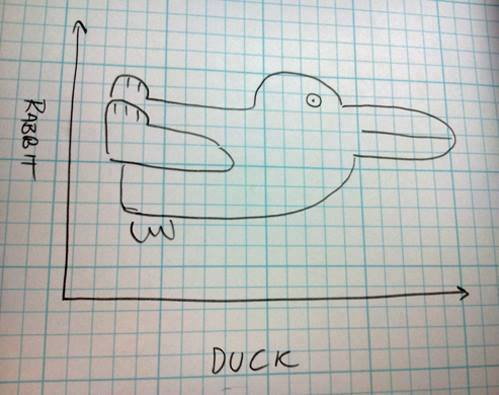
\includegraphics[width=4.0in]{rabbit-or-duck.jpg}
 }
\caption[Rabbit or duck?]
{An image that looks like a rabbit one way, and a duck another.  Your caption should describe everything that the reader sees looking at the figure, but {\it interpretation and significance} should be left for the main text.
}
\label{fig:jpgfile}
\end{figure}

\chapter{Conclusion}

I actually don't like to use "conclusion" for the final section, as it's not clear on the purpose.  I think it's better to have a "discussion" and a "summary".  In the discussion, you bring up new information by {\it interpreting} your result in the context of theory and other peoples' work; this can include new ideas and new citations.  In the summary, which will be very much like the abstract, you simply sum up your main conclusions (although the abstract, unlike the summary, has to briefly define the problem and methods).

This is where a conclusion would go.
This is where a conclusion would go.
This is where a conclusion would go.
This is where a conclusion would go.
This is where a conclusion would go.
This is where a conclusion would go.
This is where a conclusion would go.
This is where a conclusion would go.
This is where a conclusion would go.
This is where a conclusion would go.
This is where a conclusion would go.

This is where a conclusion would go.
This is where a conclusion would go.
This is where a conclusion would go.
This is where a conclusion would go.
This is where a conclusion would go.
This is where a conclusion would go.
This is where a conclusion would go.
This is where a conclusion would go.

This is where a conclusion would go.
This is where a conclusion would go.
This is where a conclusion would go.
This is where a conclusion would go.
This is where a conclusion would go.
This is where a conclusion would go.
This is where a conclusion would go.
This is where a conclusion would go.

\appendix
\chapter{Some Ancillary Stuff}

Ancillary material should be put in appendices.  The guidelines are not
clear whether bibliography comes before or after the appendices, but they
\emph{suggest} appendices come first.
Ancillary material should be put in appendices.  The guidelines are not
clear whether bibliography comes before or after the appendices, but they
\emph{suggest} appendices come first.
Ancillary material should be put in appendices.  The guidelines are not
clear whether bibliography comes before or after the appendices, but they
\emph{suggest} appendices come first.
Ancillary material should be put in appendices.  The guidelines are not
clear whether bibliography comes before or after the appendices, but they
\emph{suggest} appendices come first.

%\nocite{*}

\bibliography{magnetism}

%\begin{thebibliography}{999}
%\bibitem{spa02}E. T. Sepp\"{al}\"{a}, A. M. Pulkkinen, and M. J. Alava,
%Phys.\ Rev.\ B {\bf 66}, 144403 (2002).
%\end{thebibliography}

\end{document}
